\chapter{Processos e threads}\label{cap:ProcessosThreads}

Processo é a abstração mais conhecida no sistema operacional, trata-se de ser uma execução de um programa, além que tudo depende deste conceito para  dar suporte a possibilidade de haver operações concorrentes mesmo quando existe apenas uma \emph{CPU} disponível, através dessa abstração é possível criar um suporte a \emph{CPU}   transformando uma única \emph{CPU}  em múltiplas \emph{CPUs}  virtuais \cite{Tanenbaum2016}, \cite{info2020}, \cite{Morimoto2011}. 


\section{Processos}\label{sec:Processos}

Os computadores modernos frequentemente realizam várias tarefas ao mesmo tempo, as vezes isso é tão imperceptível que nem pensamos nisso durante a utilização de um computador, quando nao temos vários softwares abertos raramente pensamos que o sistema operacional abriu vários software de apoio ao usuário como drivers e software de GUI entre outros \cite{Tanenbaum2016}.\\
Todos os softwares executáveis no computador, às vezes incluindo o sistema operacional, são organizados em uma série de processos sequenciais, ou, simplesmente, processos. um processo é uma instância do software em execução.  durante a execução de processos temos a impressão que todos estão sendo executados simultaneamente mas esse é uma ideia errônea a cpu trabalha de forma linear processando processo a processo distintamente. o que pode acontecer é que durante o tempo de carregamento de uma informação vinda do HD que pode levar menos de 1 milisegundo para o processador esse tempo é uma eternidade e durante esse tempo de carregamento da informação ele consegue executar diversas informações \cite{Tanenbaum2016}.\\
Na verdade é como se como se cada processo possui  uma cpu virtual própria  pois a CPU real troca a todo momento de processo em processo, mas, para compreender o sistema, é muito mais fácil pensar a respeito de uma coleção de processos sendo executados em (pseudo) paralelo do que tentar acompanhar como a CPU troca de um programa para o outro \cite{Tanenbaum2016}.\\
Todos os processos devem ter suas informações salvas, cada processo pode ter diversos arquivos abertos e esse arquivos possuem ponteiros referindo ao processo, sempre que o processo retorna a execução o sistema chama o read para ler as posições salvas. quando o dados não estão em espaço de endereçamento eles são salvos na tabela de processos \cite{Tanenbaum2016}.

\begin{itemize}[label=$-$]
	\item Um sistema operacional possui três tipos de processo:
    \begin{enumerate}
        \item Execução – Um processo que realmente está sendo utilizado naquele
        instante.
        \item Pronto – Parado temporariamente para dar espaço a outro processo,
        porém é executável.
        \item • Bloqueado – Impossibilitado de executar enquanto evento externo
        esperado não acontecer
    \end{enumerate}
\end{itemize}

\begin{figure}[htpb]
    \centering
   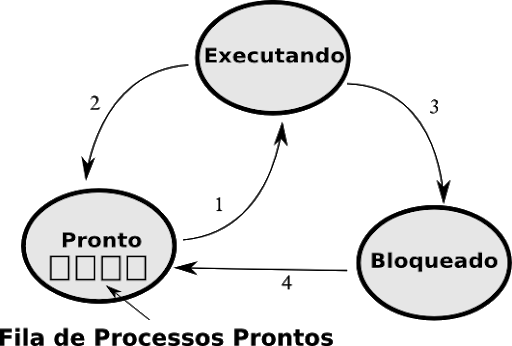
\includegraphics[scale=.4]{imagens/processso.png}
   \caption{ Estados do processo. \cite{Tanenbaum2016}}
   \label{fig:processo}
\end{figure}

\subsection{Criando processos}

Em suma os SO precisam de uma maneira de criar os processos. Podemos dizer de forma abstrata que o programa é como um livro de receita e que o processo é o ato de cozinhar em si onde se segue passo a passo da receita e que os ingredientes para o preparo são dos dados \cite{Tanenbaum2016}, \cite{info2020}, \cite{Morimoto2011}.\\
Em sistemas simples ou embarcados pode ser possível ter todos os processos que serão em algum momento necessários quando o sistema for ligado \cite{Tanenbaum2016}, \cite{info2020}, \cite{Morimoto2011}.\\
Mas para sistemas para fins gerais, no entanto, de alguma maneira é necessária para criar e terminar processos, na medida do necessário, durante a operação \cite{Tanenbaum2016}, \cite{info2020}, \cite{Morimoto2011}.\\

\begin{itemize}[label=$-$]
	\item Quatro eventos principais fazem com que os processos sejam criados:
    \begin{enumerate}
        \item Inicialização do sistema.
        \item Execução de uma chamada de sistema de criação de processo por um processo em execução.
        \item Solicitação de um usuário para criar um novo processo.
        \item Início de uma tarefa em lote. 
    \end{enumerate}
\end{itemize}

Durante o carregamento inicial do SO diversos processos são criados alguns em primeiro plano e outros em segundo plano. Podemos dizer que todos os processos de primeiro plano são de interação com o usuário e que os processo de segundo plano são de domínio do próprio sistema \cite{Tanenbaum2016}, \cite{info2020}, \cite{Morimoto2011}, \cite{Man2020}.\\
No linux server cada processo possui um número de PID (Process Identifier - em portugues Identificador de Processo)este é um número de identificação que o sistema dá a cada processo. Para cada novo processo, um novo número deve ser atribuído, ou seja, não se pode ter um único PID para dois ou mais processos ao mesmo tempo \cite{Tanenbaum2016}, \cite{info2020}, \cite{Morimoto2011}, \cite{Man2020}.\\
Os sistemas baseados em Unix precisam que um processo já existente se duplique para que a cópia possa ser atribuída a uma tarefa nova. Quando isso ocorre, o processo "copiado" recebe o nome de "processo pai", enquanto que o novo é denominado "processo filho". É nesse ponto que o PPID (Parent Process Identifier - em portugues Identificador de processo pai ) passa a ser usado: o PPID de um processo nada mais é do que o PID de seu processo pai \cite{Tanenbaum2016}, \cite{info2020}, \cite{Morimoto2011}, \cite{Man2020}.\\
No UNIX, há apenas uma chamada de sistema para criar um novo processo: fork. Essa chamada cria um clone exato do processo que a chamou. Após a fork, os dois processos, o pai e o filho, têm a mesma imagem de memória, as mesmas variáveis de ambiente e os mesmos arquivos abertos. E isso é tudo. Normalmente, o processo filho então executa execve ou uma chamada de sistema similar para mudar sua imagem de memória e executar um novo programa  \cite{Tanenbaum2016}, \cite{info2020}, \cite{Morimoto2011}, \cite{Man2020}.

\subsection{Término de processos}

Após criado o processo ele começa a ser executado e realiza qualquer que seja o seu trabalho, e como pode se imaginar pouco depois ele tende a ser finalizado.

\begin{itemize}[label=$-$]
	\item O novo processo terminará, normalmente devido a uma das condições a seguir:
    \begin{enumerate}
        \item Saída normal (voluntária)
        \item Erro fatal (involuntário). 
        \item Saída por erro (voluntária). 
        \item Morto por outro processo (involuntário). 
    \end{enumerate}
\end{itemize}

A maioria dos processos ele termina por ter chegado ao seu final, ou seja, quando um compilador termina de traduzir o programa dado a ele, o compilador executa uma chamada para dizer ao sistema operacional que ele terminou. A segunda é um erro fatal por exemplo a execução de um arquivo que nao existe no sistema. A terceira possibilidade é quando existe um erro no programa executado por algum tipo de dado inexistente ou incorreto \cite{Tanenbaum2016}, \cite{info2020}, \cite{Morimoto2011}, \cite{Man2020}
A quarta razão é quando o processo sofre influência externa por exemplo por um comando que finalize esse processo. Esse motivo em especial existe uma grande variação de comandos linux para executar esse tipo de recurso em especial o comando kill \cite{Tanenbaum2016}, \cite{info2020}, \cite{Morimoto2011}, \cite{Man2020}

O comando kill envia o sinal especificado para o especificado processos ou grupos de processos.
Se nenhum sinal for especificado, o sinal termino é enviado. O padrão ação para este sinal é encerrar o processo. Este sinal deve ser usado de preferência ao sinal KILL, uma vez que um     processo pode instalar um manipulador para o sinal termino a fim de executar etapas de limpeza antes de encerrar de maneira ordenada. Se um o processo não termina depois que um sinal termino foi enviado, então o sinal KILL pode ser usado; esteja ciente de que o último sinal não pode   ser capturado e, portanto, não dá ao processo de destino a oportunidade de execute qualquer limpeza antes de encerrar \cite{Tanenbaum2016}, \cite{info2020}, \cite{Morimoto2011}, \cite{Man2020}
A maioria dos shells modernos tem um comando kill embutido , com um uso semelhante ao do comando descrito aqui. As opções --all , --pid e --queue e a possibilidade de especificar processos por comando nome, são extensões locais \cite{Tanenbaum2016}, \cite{info2020}, \cite{Morimoto2011}, \cite{Man2020}
Caso prefira, você também pode matar de uma vez só todos os comandos selecionado ao nome de um programa. Para isso, basta usar o comando killall seguido do nome do software em questão, como killall vim \cite{Tanenbaum2016}, \cite{info2020}, \cite{Morimoto2011}, \cite{Man2020}
Porém, o killall exige uma certa rigidez ao informar o nome do processo. Caso você não tenha certeza do nome completo, pode tentar o pkill, que faz diversas associações com a palavra-chave digitada \cite{Tanenbaum2016}, \cite{info2020}, \cite{Morimoto2011}, \cite{Man2020}



\newpage
\section{Threads}\label{sec:Threads}


Cada programa, ou processo, possui normalmente um fluxo de controle. Assim o programa é executado seqüencialmente passo a passo com seu único fluxo de controle. Em sistemas operacionais tradicionais, cada processo tem um espaço de endereçamento e um único \emph{thread} de controle. Neste ponto que as \emph{threads} se destacam, com as \emph{threads} podemos ter mais de um único fluxo de controle em nosso aplicativo \cite{Tanenbaum2016}, \cite{dev2020}.\\
As \emph{threads} em  muitas situações, é desejável ter múltiplos \emph{threads} de controle no mesmo espaço de endereçamento executando em quase paralelo, como se eles fossem (quase) processos separados (exceto pelo espaço de endereçamento compartilhado) \cite{Tanenbaum2016}, \cite{dev2020}.\\
Assim o \emph{software} agira como se tivessem sido dividido em varias partes de seu código atuando em paralelo no sistema. \emph{Threads} são, portanto, entidades escalonadas para executarem na \emph{CPU}, por isso a noção de (pseudo) paralelismo, pois as \emph{threads} concorrerão pelo processador juntamente com mais \emph{threads} que tiverem no programa, ou concorrerá apenas com o fluxo do programa \cite{Tanenbaum2016}, \cite{dev2020}.


\newpage
\section{Escalonamento}\label{sec:Escalonamento}

O escalonador é um subsistema do SO encarregado de direcionar a prioridade de entrada dos processos na CPU. os algoritmos avaliam o cenário disposto pelo sistema e com isso determina a lógica empregada para resolver qual processo será processado é importante lembrar que algumas variáveis necessitam de mais processo estes ocuparão a CPU por um tempo maior e não precisam da intervenção do usuário. Os processos que precisam de mais entradas e saídas de dados, ou seja, o processo demanda intervenção do usuário \cite{Tanenbaum2016}.
\begin{figure}[htpb]
    \centering
   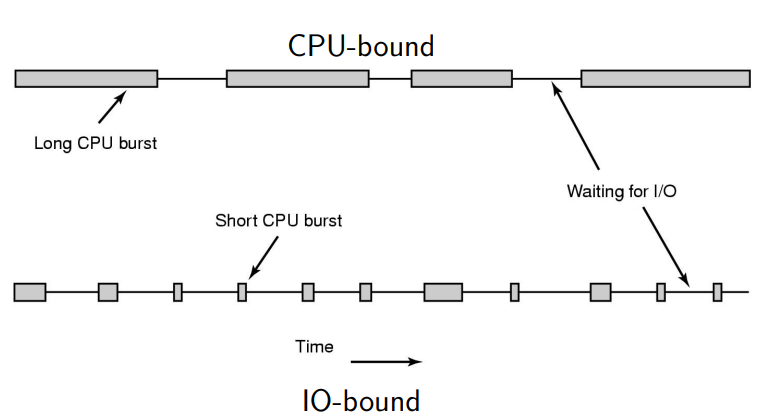
\includegraphics[scale=.4]{imagens/escalonamento1.png}
   \caption{Comportamento de processos. \cite{Tanenbaum2016}}
   \label{fig:escalonador}
\end{figure}

\subsection{Categorias de algoritimo de escalonamento}

Diferentes algoritmos de escalonamento são implementados para tratar condição que acontece nas diferentes áreas de aplicação do SO principalmente processos identificados para objetivos diferentes. Cada sistema tem particularidades que devem ser levadas em consideração pelo escalonador \cite{Tanenbaum2016}.

\begin{itemize}[label=$-$]
	\item É necessário distinguir três ambientes:
    \begin{enumerate}
        \item Lote
        \item Interativo
        \item Tempo real 
    \end{enumerate}
\end{itemize}

Sistema em lote são bastante comuns por sua otimização no tempo de retorno e maximiza o número de horas de trabalho e muitas vezes aplicáveis a outras situações também, o que torna seu estudo interessante, mesmo para pessoas não envolvidas na computação corporativa de grande porte \cite{Tanenbaum2016}.

Sistemas interativos tem objetivo de otimizar o tempo de resposta, mesmo que nenhum processo execute de modo intencional para sempre, um erro em um programa pode levar um processo a impedir indefinidamente que todos os outros executem.Os servidores Linux também caem nessa categoria, visto que eles normalmente servem a múltiplos usuários (remotos), todos os quais estão muito apressados, assim como usuários de computadores \cite{Tanenbaum2016}.

Em sistemas de tempo real, os processos sabem que eles não podem executar por longos períodos e em geral realizam o seu trabalho e bloqueiam rapidamente. A diferença com os sistemas interativos é que os de tempo real executam apenas programas que visam ao progresso da aplicação à mão \cite{Tanenbaum2016}.
% \section{Comunicação entre processos}\label{sec:ComProc}